\chapter{Characterizing Radio Energy Usage of Smartphones in Cellular Networks} 
\label{chap:power}

Smartphones with cellular data access have become increasingly popular across the globe, with the wide deployment of 3G and emerging LTE~\cite{3gpp.lte} networks, and a plethora of applications of all kinds. Cellular networks are typically characterized by limited radio resources and significant device power consumption for network communications. The battery capacity of smartphones cannot be easily improved due to physical constraints in size and weight. Hence, battery life remains a key determinant of end-user experience. Given the limited radio resources in these networks and device battery capacity constraints, optimizing the usage of these resources is critical for cellular carriers and application developers. Specifically, radio power is reported to be 1/3 to 1/2 of the total device power~\cite{mobisys.aro}, and in this chapter, we first devise a systematic way to characterize smartphone radio energy usage given packet traces as input and then we discuss our analysis results with real user traces.

\nsection{Power Measurement Methodology}
\label{sec:power.method}

Similar to previous studies~\cite{imc.3g, codes.powertutor}, we use Monsoon power monitor~\cite{monsoon} as power input for our device measuring power traces at the same time. The power trace contains two fields, timestamp and average instant power, and the sampling rate is 5000Hz. The test device is an HTC phone with LTE data plan from a cellular ISP. It has 768 MB RAM memory and 1 GHz Qualcomm MSM8655 CPU, running Android 2.2.1. We remove the battery and connect $\oplus$ and $\ominus$ pins of the power monitor to device's $\oplus$ and $\ominus$ pins, respectively. By enabling $V_{out}$ with the voltage of 3.7V, the device boots properly and the power monitor records the total power traces consumed by the device. Another tricky part for our setup is that, the back cover of our test device, HTC Thunderbolt, must remain attached firmly, otherwise, if it is pried off the device, LTE session is terminated and 1xRTT session is started. This is because part of the LTE antenna circuit lies inside the back cover~\cite{thunderbolt}. In the end, we let the wires going out of the back cover through the hole of earplugs.

%In Section~\ref{sec:background.power},  Figure~\ref{fig:trace.all} and Figure~\ref{fig:trace.zoom} visualize one such power measurement in LTE network.
We share the same observation with previous study~\cite{codes.powertutor} that screen plays an important role in device power consumption, \ie with screen 100\% on, the UE idle power is 847.15mW compared with 11.36mW with screen off. For all measurements, we keep the test application running in the background with screen completely off to minimize power noise, unless UI interactions are required and screen should be kept on, \ie measuring power for browser. In this case, we subtract screen power from the total, with slightly increased noise. All experiments are repeated at least 5 times to reduce measurement error.

To measure state transition power levels, UE keeps a long-lived TCP connection with the server and packet traces are collected to make sure there is no background traffic. In order to trigger state promotions, we make the device idle for sufficient time, \eg 30 seconds, and then send a packet from server to client. UE remains idle afterwards and demotes to idle state in the end, and the power trace covers the full tail.

\nsection{Smartphone Power Model}

In Section~\ref{sec:bkg.rrc}, we have discussed the radio resource control mechanisms in cellular network. In fact, RRC state machine is the key factor for determining the UE power consumption for both 3G and LTE 4G networks.

In this section, we take LTE network as a sample and illustrate the power traces of our test Android smartphone in a commercial LTE network based on local experiments. We observe that network activities match the corresponding state transitions indicated by different power levels.

\begin{figure}[t]
\centering
\IG{figures/mobisys12/trace_all.eps} \\
\ncaption{Power states of LTE}
\label{fig:trace.all}
\end{figure}

%So the plot of power traces in Figure 3 consists of dots of readings and may be >>594mW. During the DRX in RRC_IDLE, the actual power curve is something like a "n" shape curve (an increase period, a fluctuating top, and a decrease period). The average of the whole on period is 594mW, but the pikes inside the on period can be >>594mW. Those spikes have very minor effect in the energy calculation, but they are very obvious to see in the power trace figure.

Figure~\ref{fig:trace.all} shows the power trace of uploading at the speed of 1Mpbs for 10 seconds. With screen off, the energy is mostly consumed by the radio interfaces, as the power level is less than 20mW before $t_1$. At $t_1$, the application sends a TCP {\sf SYN} packet triggering \RI to \RC promotion, and the application waits for $T_{pro}$ until starting data transfer at $t_2$. Between $t_2$ and $t_3$, depending on the instant data rate, the power level fluctuates. We notice the power level during fast data transfer is significantly higher than the base power in \RC, which motivates us to incorporate data rates into our LTE power model. After the data transfer completes at $t_3$, the device remains in \RC for a fixed tail time $T_{tail}$, until $t_4$, when the device goes back to \RI. The periodicity of DRX between $t_3$ and $t_4$ is not obvious due to limited sample rate.

%If there is any data sent or received between $t_3$ and $t_4$, the tail timer gets reset and a new tail starts.

\begin{figure}[h]
\centering
\IG{figures/mobisys12/trace_zoom.eps} \\
\ncaption{Zoom-in view in \RC}
\label{fig:trace.zoom}
\end{figure}

Figure~\ref{fig:trace.zoom} is a 125$\times$ zoom-in view of Figure~\ref{fig:trace.all}'s tail, which clearly illustrates DRX activity in \RC~mode. The device activates its receivers to listen to downlink control channel. If downlink traffic is found awaiting, the device goes into Continuous Reception model; otherwise, the device goes into a dormant state without continuously checking downlink control channel, though still remaining in \RC~mode. The spikes appearing every 40 ms in Figure~\ref{fig:trace.zoom} match the on period of DRX in \RC.



\nsection{Power Model Construction}
This section summarizes the construction of the new LTE power model, as well as the 3G and WiFi model measured from the same LTE phone. We then compare energy efficiency in bulk data transfer for different networks and validate LTE power model in the end.

\begin{table}[t]
\begin{center}
\begin{tabular}{|c|c|c|c|c|}\hline
 & Power$^\star$ & Duration & Periodicity\\
 & (mW) & (ms) & (ms)\\\hline\hline
Screen off (base) & 11.4$\pm$0.4 & N/A & N/A\\\hline
Screen 100\% on & 847.2$\pm$2.7 & N/A & N/A\\\hline\hline
 
\MR{LTE promotion} & \MR{1210.7$\pm$85.6} & $T_{pro}$: & \MR{N/A} \\
 &  &  260.1$\pm$15.8 & \\\hline
%it's not continuous reception since there is 40ms DRX
LTE Short DRX On & \MR{1680.2$\pm$15.7} & $T_{on}$: & $T_{ps}$:\\
\RC & & 1.0$\pm$0.1 & 20.0$\pm$0.1 \\\hline
LTE Long DRX On & \MR{1680.1$\pm$14.3} & $T_{on}$: & $T_{pl}$:\\
\RC & & 1.0$\pm$0.1 & 40.1$\pm$0.1 \\\hline
\MR{LTE tail base} & \MR{1060.0$\pm$3.3} & $T_{tail}$: & \MR{N/A} \\
 &  & 11576.0$\pm$26.1 & \\\hline
LTE DRX On & \MR{594.3$\pm$8.7} & $T_{oni}$: & $T_{pi}$:\\
\RI &  & 43.2$\pm$1.5 & 1280.2$\pm$7.1\\\hline\hline

3G promotion & 659.4$\pm$40.4 & 582.1$\pm$79.5 & N/A \\\hline
3G DCH tail base & 803.9$\pm$5.9 & 8088.2$\pm$149.6 & N/A \\\hline
3G FACH tail base & 601.3$\pm$6.4 & 824.2$\pm$148.1 & N/A \\\hline
3G DRX (idle) & 374.2$\pm$13.7 & 55.4$\pm$1.5 & 5112.4$\pm$37.7 \\\hline\hline

WiFi promotion & 124.4$\pm$2.6 & 79.1$\pm$15.1 & N/A \\\hline
WiFi tail base & 119.3$\pm$2.5 & 238.1$\pm$9.2 & N/A \\\hline
WiFi beacon (idle) & 77.2$\pm$1.1 & 7.6$\pm$0.1 & 308.2$\pm$1.0 \\\hline
\end{tabular}
\ncaption{LTE, 3G, and WiFi power model}
\label{tab:power}
\begin{tabular}{l}
\\{$^\star$All power readings in this table include the base power (screen off),}\\
{~~which has negligible impact on total energy.}
\end{tabular}
\end{center}
\end{table}

\nsubsection{Power model for RRC and DRX}
\label{sec:power.rrc}

With the experimental setup described in Section~\ref{sec:power.method}, we measure power model for LTE, 3G, and WiFi on the LTE phone, summarized in Table~\ref{tab:power}. The LTE parameter values are validated by the network-based measurement in Section~\ref{sec:net.sm}\comment{update reference}. For simplicity, we ignore the WiFi AP scanning and association, assuming UE is already connected with an AP.

First, we observe that LTE reduces the promotion delay ($T_{pro}$) from 3G's 582.06ms to 260.13ms. However, the power level is almost doubled, \ie 1210.74mW (LTE) v.s. 659.43mW (3G). WiFi has the most lightweight state promotion with smaller $T_{pro}$ and much lower power level.

Secondly, LTE appears to have longest tail (11.576 seconds) with highest tail base power (1060.04 mW). Summing up DCH and FACH tail, 3G's total tail time (8.9 seconds) is smaller than LTE's $T_{tail}$ of 11.6 seconds. Even 3G DCH's tail base power is 24.17\% lower than LTE's tail base power, and the gap becomes 25.25\% if we consider LTE DRX in \RC with a high on duration power (1680.20mW). WiFi is much more power efficient, with shorter tail and much lower base power.

We also compare LTE DRX in \RI~with 3G DRX and WiFi beacon in the idle state. LTE has the highest on power and slightly smaller On Duration than 3G, while WiFi has smallest on power and On Duration. The cycle of LTE (1.28 seconds) is in between 3G and WiFi.

Based on these observations, LTE is less energy efficient during idle state and for transferring smaller amount of data. For example, if only one packet is transferred, the energy usage considering both promotion and tail energy for LTE, 3G and WiFi is 12.76J, 7.38J and 0.04J, respectively. One possible reason for LTE's higher power states is that devices must incorporate {\em multiple-input and multiple-output} (MIMO) to support LTE network, \eg the test device we use has 1 transmit antenna and 2 receive antennas, which contributes to higher power consumption.

\begin{figure*}[tp]
\centering
\begin{minipage}[b]{.49\textwidth}
\centering
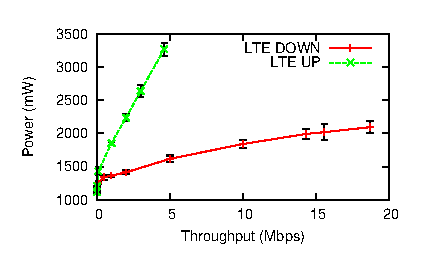
\includegraphics[width=.99\textwidth]{figures/mobisys12/power_tp.eps}
\ncaption{\small Power-throughput curve for LTE network}
\label{fig:power.tp}
\end{minipage}
\begin{minipage}[b]{.49\textwidth}
\centering
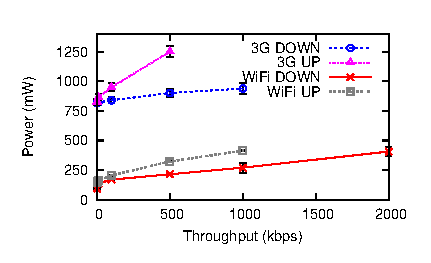
\includegraphics[width=.99\textwidth]{figures/mobisys12/power_tp2.eps}
\ncaption{\small Power-throughput curve for 3G and WiFi}
\label{fig:power.tp2}
\end{minipage}
\end{figure*}

\begin{figure}[t]
\centering
\IG{figures/mobisys12/up_down.eps} \\
\ncaption{Power of simultaneous uplink and downlink transfers}
\label{fig:up.down}
\end{figure}



\nsubsection{Power model for data transfer}
\label{sec:updown}
Previous work on 3G UMTS power modeling either treats DCH power state to have a fixed power value~\cite{codes.powertutor, mobisys.aro}, or assumes energy per bit to be the same constant for both uplink and downlink~\cite{imc.tailender}. These assumptions might be reasonable given that 3G has relatively low data rates. However, for LTE, we observe that device power is much higher during high speed data transmission (up to 3300mW for uplink) relative to the base power (1060mW) in \RC, and there is significant difference between downlink and uplink power levels at the same data rate. In this paper, we propose a new comprehensive power model for LTE empirically derived in a commercial LTE network.

We start with measuring device power states with controlled uplink or downlink throughput. The impact of TCP {\sf ACK} packets, which are small in size, is minor, thus ignored.

%TCP uplink data transfer incurs ACK packets in downlink direction, and vise versa. However, the impact of ACK packets is minor, which are smaller and fewer than data packets and the number of ACK packets.

Figures~\ref{fig:power.tp} and~\ref{fig:power.tp2} present the power-throughput curve for LTE, 3G, and WiFi. The curves are limited by the peak data rate we can achieve at the test location.
We observe that for all networks, a linear model fits well for both uplink and downlink. Assume uplink throughput is $t_u$ (Mbps) and downlink throughput is $t_d$ (Mbps), the power level (mW) for uplink is $P_u = \alpha_u t_u + \beta$ and for downlink $P_d = \alpha_d t_d + \beta$.
The best fit parameters are listed in Table~\ref{tab:up.down}.

\begin{table}[t]
\begin{center}
\begin{tabular}{|c|c|c|c|c|}\hline
 & $\alpha_u$ (mW/Mbps) & $\alpha_d$ (mW/Mbps) & $\beta$ (mW) & $\alpha_u/\alpha_d$ \\\hline
LTE & 438.39 & 51.97 & 1288.04 & 8.44\\\hline
3G & 868.98 & 122.12 & 817.88 & 7.12\\\hline
WiFi & 283.17 & 137.01 & 132.86 & 2.07\\\hline
\end{tabular}
\ncaption{Data transfer power model}
\label{tab:up.down}
\end{center}
\end{table}

By looking at $\alpha_u/\alpha_d$, we notice that uplink power increases faster than downlink for all three networks types. This is expected because sending data requires more power than receiving data for wireless data access~\cite{ieee.mimo}. LTE has the largest gap of $\alpha_u/\alpha_d = 8.44$ among three network types. This is largely because $\alpha_d$ for LTE is quite small. For 3G, both $\alpha_u$ and $\alpha_d$ are larger than LTE. $\beta$ is the base power when throughput is 0, with the ranking of LTE $>$ 3G $>$ WiFi. This is consistent with the tail base power comparison in Table~\ref{tab:power}. We notice that $\beta$ is slightly higher than the tail base for all networks types. This is possibly because of the overhead of switching transmitters or receivers into high speed mode.



For simultaneous uplink and downlink transfers, given that transmitters and receivers are separate, we conjecture that the power level (mW) is given by the following formula:
\begin{equation*}
P = \alpha_u t_u + \alpha_d t_d+ \beta
\end{equation*}
To validate this conjecture, we measure the power levels for concurrent uplink and downlink transfers in Figure~\ref{fig:up.down}. Assume total throughput $t = t_u + t_d$ and the ratio of uplink throughput $\epsilon = t_u \big/ t$:
\begin{equation*}
P = \alpha_u t_u + \alpha_d t_d+ \beta = (\alpha_u - \alpha_d)t\epsilon + \alpha_d t + \beta
\end{equation*}
When $t$ is a constant, $P$ grows linearly with $\epsilon$ and the slope is $(\alpha_u - \alpha_d)t$. Figure~\ref{fig:up.down} shows two curves of $t = 1$Mbps and $t = 2$Mbps, both having a strong linear pattern and the slope is less than 5\% off the expected value.


\nsubsection{Energy efficiency for bulk data transfer}
\label{sec:power.bulk}

\begin{figure}[t]
\centering
\IG{figures/mobisys12/energy_size.eps} \\
\ncaption{Energy per bit for bulk data transfers}
\label{fig:energy.size}
\end{figure}

To compare the power efficiency of different networks in the wild, we use bulk data transfer experiments to measure energy per bit.
Perrucci \etal~\cite{vtc.survey} measure energy per bit for 3G and WiFi with a fixed bulk size. In addition to taking LTE into consideration, we vary the bulk size to cover more possible network usage scenarios. Figure~\ref{fig:energy.size} shows the measured energy per bit in $\mu J / bit$ ($10^{-6} Joule / bit$) with different bulk data size. All data is randomly generated so that there is no chance for caching. We do not include promotion or tail energy but instead focus on data transfer energy. Given that signal strength and peak data rate on wireless networks fluctuates, both affecting energy per bit, our measurement only serves as a sampled view for the energy efficiency of different networks.
%\comment{why cite this study only?  it's the closest to ours?}

First, energy per bit decreases as bulk data size increases, largely because with a small data size, throughput does not reach link capacity due to TCP slow start. We also observe that LTE's energy per bit in downlink is comparable with WiFi, although the absolute power level of LTE is much higher than WiFi. This is due to high downlink throughput for LTE at our test location, even compared with the WiFi network. Similarly, for LTE uplink, it drops from 10$\mu J / bit$ to less than 1$\mu J / bit$ as bulk data size increases. With bulk data size of 10MB, LTE consumes 1.62 times the energy of WiFi for downlink and 2.53 for uplink. With lowest throughput, 3G has the worst energy efficiency for large data transfer, \eg for downloading 10MB data, 3G requires 21.50 times the energy of LTE and 34.77 times the energy of WiFi, and for uplink, 7.97 times of LTE and 20.16 times of WiFi.

%3G and LTE require 34.77 and 1.62 times the energy of WiFi, respectively, and for uplink, 3G/WiFi ratio is 20.16 and LTE/WiFi ratio is 2.53.
%\comment{I thought these numbers are interesting and should be included in the intro: in particular, you should have small transfer (1 packet) vs. bulk transfer energy per bit comparision}

\nsubsection{Power model validation}
\label{sec:power.validation}

\begin{table}[h]
\begin{center}
\begin{tabular}{|c|c|c|c|c|}\hline
\MR{App} & Measured & Simulated & \MR{Error}  \\
&energy (J)\footnotemark[1] & energy (J)\footnotemark[1] &\\\hline
Website G\footnotemark[3] & 24.77 & 24.37 & -1.61\% (-2.06\%\footnotemark[2]) \\\hline
Website Y\footnotemark[3] & 31.84 & 30.08 & -5.53\% (-7.04\%) \\\hline
YouTube & 21.81 & 21.14 & -3.07\% (-4.17\%) \\\hline
NPR News & 24.65 & 24.37 & -1.12\% (-1.70\%) \\\hline
Market & 38.64 & 38.03 & -1.58\% (-3.03\%) \\\hline
\end{tabular}
\\
\begin{tabular}{l}
{$^1$Both measured and simulated energy include tail energy}\\
{$^2$This error is for simulated energy assuming $\alpha_u = \alpha_d = 0$}\\
{$^3$Refer to \S\ref{sec:method.app}\comment{update reference} for the definition of \WG and \WY}\\
\end{tabular}
\ncaption{LTE power model validation}
\label{tab:power.validation}
\end{center}
\end{table}

To validate the LTE power model and the trace-driven simulation (\S\ref{sec:method.sim}), we compare measured energy (measured from the LTE phone) with simulated energy for case study applications. Table~\ref{tab:power.validation} contains the sample application usage scenarios described in \S\ref{sec:method.app}. The error rate is consistently less than 6\%, with the largest error rate from \WY, which includes heavy JavaScript execution and HTML rendering. Since our power model focuses on radio power and ignores the impact of CPU, for \WY, the total energy usage is slightly underestimated. 
%As we observe, the impact of non-network components on total energy is minor, except for the excluded screen. 

The error rate is increased if the impact of downlink and uplink throughput is ignored, \ie assuming $\alpha_u = \alpha_d = 0$. However, the increase is not significant, at most 1.5\%. This is because for these web-based applications, network throughput is low due to small object size (\S\ref{sec:app.perf}\comment{update reference}). For other applications, such as video/audio streaming and file download, we expect to see a larger gap in error rate if the impact of downlink/uplink is ignored.

In this section, in addition to comparing energy per bit in bulk data transfer for different networks, we construct a new LTE power model and validate its accuracy, which is the basis for the following analysis.


\nsection{User Trace Based Tradeoff Analysis}

\nsubsection{trace-driven network/power simulation methodology (validation)}
\S3.3

\nsubsection{\S6.1, 6.2, 6.3}
